\section{}
% A 50 mm square plate is subjected to the stresses as shown in Fig. 4. What deformation is
% experienced by diagonal BD? Determine the stress on planes perpendicular and parallel to BD
% and then employ generalized Hooke’s law [Eqn. (2)]. Express the solution in terms of E for
% v = 0.3.
% Figure 4: A square plate
% εx = 1
% E
% [
% σx − ν (σy + σz
% )]
% (2a)
% εy = 1
% E
% [σy − ν (σx + σz )] (2b)
% εz = 1
% E
% [
% σz − ν (σx + σy
% )]
% (2c)
%6

A $\qty{50}{\milli\meter}$ square plate is subjected to the stresses as shown in Fig. \ref{fig:fig4}. What deformation is
experienced by diagonal $\overline{BD}$? Determine the stress on planes perpendicular and parallel to $\overline{BD}$
and then employ generalized Hooke's law. Express the solution in terms of $E$ for $\nu = 0.3$.

\begin{figure}[h]
    \centering
    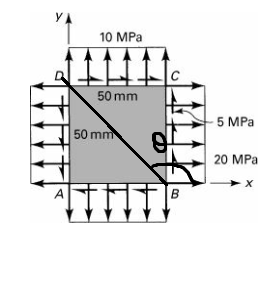
\includegraphics[width=0.3\linewidth]{Questions/Figures/Q6ProblemDiagram.png}
    \caption{A square plate}
    \label{fig:fig4}
\end{figure}

Generalized hooke's law
\begin{align*}
    \epsilon_x &= \frac{1}{E}[\sigma_x - \nu(\sigma_y + \sigma_z)] \\
    \epsilon_y &= \frac{1}{E}[\sigma_y - \nu(\sigma_x + \sigma_z)] \\
    \epsilon_z &= \frac{1}{E}[\sigma_z - \nu(\sigma_x + \sigma_y)]
\end{align*}

From the Fig. \ref{fig:fig4},
\begin{align*}
    \sigma_x &= \qty{20}{\mega\pascal} \\
    \sigma_y &= \qty{10}{\mega\pascal} \\
    \sigma_z &= \qty{0}{\mega\pascal} \\
    \tau_{xy} &= \qty{5}{\mega\pascal} \\
    \nu &= 0.3 \\
\end{align*}

The strain in the $x$ and $y$directions are:
% rewrite final answers as pressure/E
% \begin{align*}
%     \epsilon_x &= \frac{1}{E}[\sigma_x - \nu(\sigma_y + \sigma_z)] \\
%     &= \frac{1}{E}[20 - 0.3(10 + 0)] \\
%     &= \frac{1}{E}\qty{17}{\mega\pascal} \\
%     \epsilon_y &= \frac{1}{E}[\sigma_y - \nu(\sigma_x + \sigma_z)] \\
%     &= \frac{1}{E}[10 - 0.3(20 + 0)] \\
%     &= \frac{1}{E}\qty{4}{\mega\pascal} \\
%     \epsilon_z &= \frac{1}{E}[\sigma_z - \nu(\sigma_x + \sigma_y)] \\
%     &= \frac{1}{E}[0 - 0.3(20 + 10)] \\
%     &= \frac{1}{E}\qty{-9}{\mega\pascal} \\
% \end{align*}
\begin{align*}
    \epsilon_x &= \frac{1}{E}[\sigma_x - \nu(\sigma_y + \sigma_z)] \\
    &= \frac{1}{E}[20 - 0.3(10 + 0)] \\
    &= \frac{\qty{17}{\mega\pascal}}{E} \\
    \epsilon_y &= \frac{1}{E}[\sigma_y - \nu(\sigma_x + \sigma_z)] \\
    &= \frac{1}{E}[10 - 0.3(20 + 0)] \\
    &= \frac{\qty{4}{\mega\pascal}}{E} \\
    \epsilon_z &= \frac{1}{E}[\sigma_z - \nu(\sigma_x + \sigma_y)] \\
    &= \frac{1}{E}[0 - 0.3(20 + 10)] \\
    &= \frac{\qty{-9}{\mega\pascal}}{E} \\
\end{align*}

The shear strain is:
\begin{align*}
    \gamma_{xy} &= \frac{\tau_{xy}}{G} \\
    &= \frac{5}{\frac{E}{2(1+\nu)}} \\
    &= \frac{5}{\frac{E}{2(1+0.3)}} \\
    &= \frac{\qty{13}{\mega\pascal}}{E} 
\end{align*}

From the Figure, $\theta$:
\begin{align*}
    \theta &= 90 + \tan^{-1}\left(\frac{50}{50}\right) \\
    &=  \ang{135}
\end{align*}

The length of the diagonal is:
\begin{align*}
    \overline{BD} &= \sqrt{50^2 + 50^2} \\
    &= \qty{70.71}{\milli\meter}
\end{align*}

The strain in the diagonal is:
\begin{align*}
    \epsilon_{BD} &= \epsilon_x\cos^2\theta + \epsilon_y\sin^2\theta + \gamma_{xy}\sin\theta\cos\theta \\
    &= \frac{\qty{17}{\mega\pascal}}{E}\cos^2(\ang{135}) + \frac{\qty{4}{\mega\pascal}}{E}\sin^2(\ang{135}) + \frac{\qty{13}{\mega\pascal}}{E}\sin(\ang{135})\cos(\ang{135}) \\
    &= \frac{1}{E}(17\cos^2(\ang{135}) + 4\sin^2(\ang{135}) + 13\sin(\ang{135})\cos(\ang{135})) \\
    &= \frac{\qty{4}{\mega\pascal}}{E}
\end{align*}

The change in length of the diagonal is:
\begin{align*}
    \Delta L_{BD} &= \epsilon_{BD}\overline{BD} \\
    &= \frac{\qty{4}{\mega\pascal}}{E}\qty{70.71}{\milli\meter} \\
    &= \boxed{\frac{\qty{283}{\milli\meter\mega\pascal}}{E}}
\end{align*}